\paragraph{Model configuration}

\paragraph{Training}\mbox{}\\
Objective: Minimize loss function defined as:

% \paragraph{}\mbox{}\\
\paragraph{Model configuration}\mbox{}\\
\begin{table}[H]
\centering
\begin{tabular}{|l|l|}
\hline
\textbf{Parameter} & \textbf{Value} \\
\hline
\multicolumn{2}{|c|}{\textbf{Training}} \\
\hline
Batch Size & 1 \\
\hline
Seed & 42 \\
\hline
Epochs & 15000 \\
\hline
Training Ratio & 0.9 \\
\hline
Number of Nodes & 1 \\
\hline
Gradient Clip Value & 1.0 \\
\hline
Metric to Monitor & val/recon\_loss \\
\hline
Metric Mode & Min \\
\hline
Device & CUDA \\
\hline
\multicolumn{2}{|c|}{\textbf{Model}} \\
\hline
Image Channels & 1 \\
\hline
Embedding Dimension & 8 \\
\hline
Number of Codes & 16384 \\
\hline
Number of Hidden Layers & 16 \\
\hline
Learning Rate & 5e-6 \\
\hline
Downsample Factors & [2, 2, 2] \\
\hline
Discriminator Channels & 64 \\
\hline
Discriminator Layers & 3 \\
\hline
Discriminator Iteration Start & 10000 \\
\hline
Discriminator Loss Type & Hinge \\
\hline
Image GAN Weight & 1.0 \\
\hline
Video GAN Weight & 1.0 \\
\hline
L1 Weight & 4.0 \\
\hline
GAN Feature Weight & 4.0 \\
\hline
Perceptual Weight & 4.0 \\
\hline
I3D Feature & False \\
\hline
Restart Threshold & 1.0 \\
\hline
No Random Restart & False \\
\hline
Normalization Type & Group \\
\hline
Padding Type & Replicate \\
\hline
Number of Groups & 32 \\
\hline
\multicolumn{2}{|c|}{\textbf{Dataset}} \\
\hline
Caching & Disk \\
\hline
Path & /ravana/d3d\_work/micorl/data/ct\_images\_prostate\_32fixed/ \\
\hline
Image Size & 128 \\
\hline
Number of Slices & 32 \\
\hline
Window Width & 400 \\
\hline
Window Level & 60 \\
\hline
\end{tabular}
\caption{Parameters for the Meta VQGAN}
\label{table:meta_vqgan_params}
\end{table}

\paragraph{Training}\mbox{}\\

\begin{figure}[H]
\minipage{0.49\textwidth}
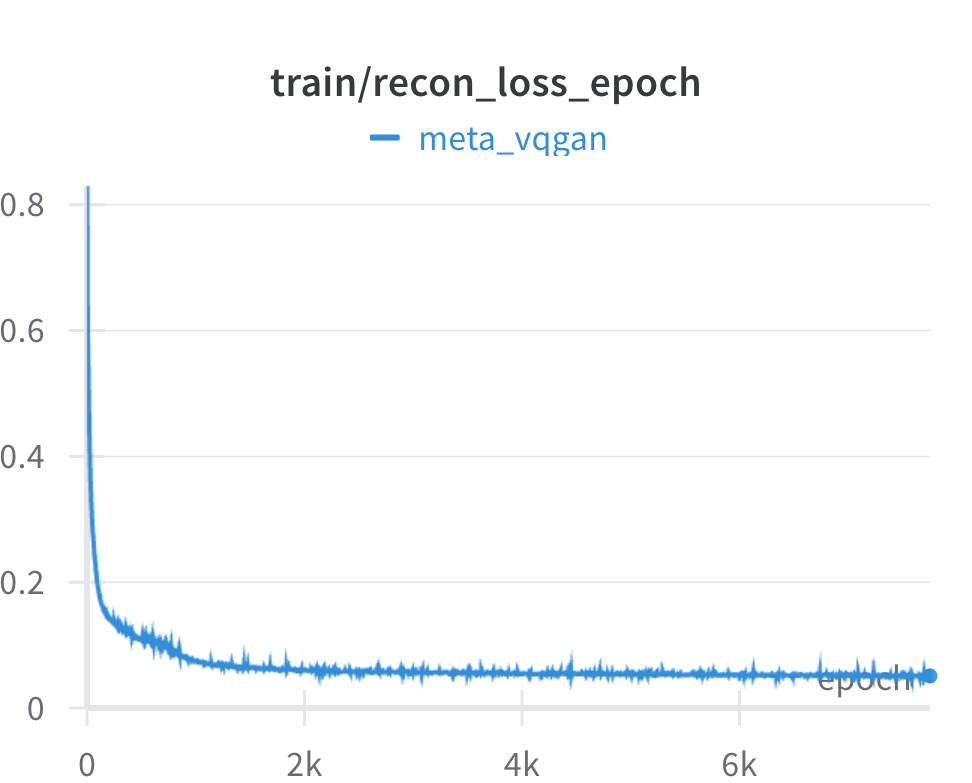
\includegraphics[width=\linewidth]{detailed_engineering/Meta VQGAN/charts/Section-2-Panel-13-1qhe42yar.png}
\caption{Reconstruction loss during the training.}
\endminipage\hfill
\minipage{0.49\textwidth}
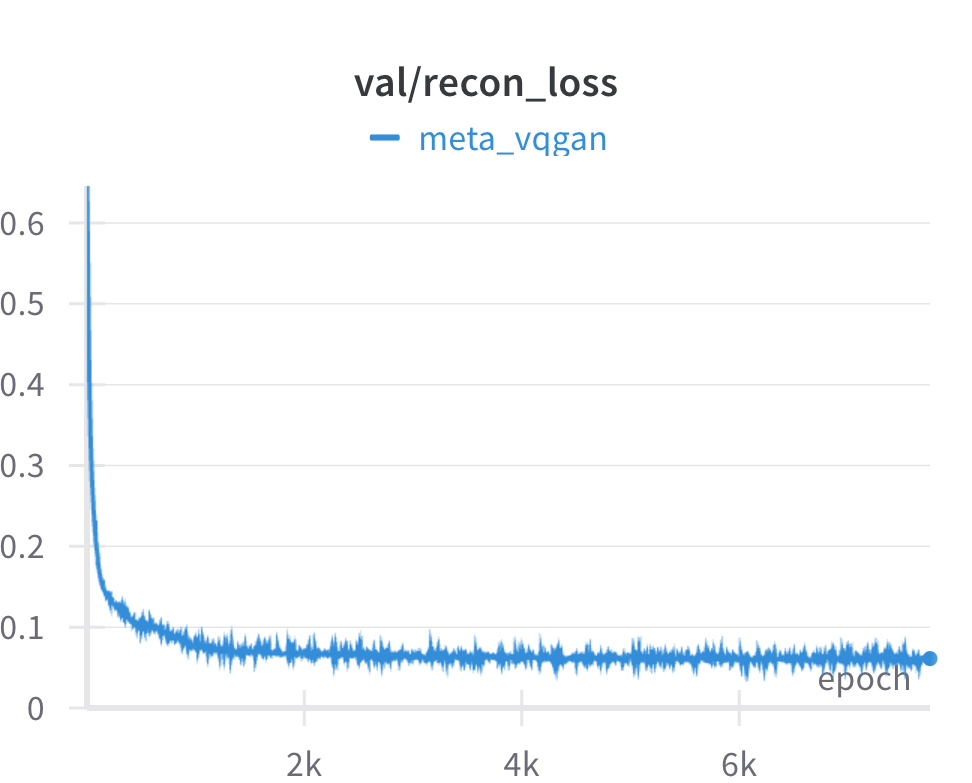
\includegraphics[width=\linewidth]{detailed_engineering/Meta VQGAN/charts/Section-4-Panel-3-hkj1c12xb.png}
\caption{Reconstruction loss during the validation.}
\endminipage
\caption{Reconstruction loss during the training and the validation. Lower is better.}
\end{figure}

\begin{figure}[H]
\minipage{0.49\textwidth}
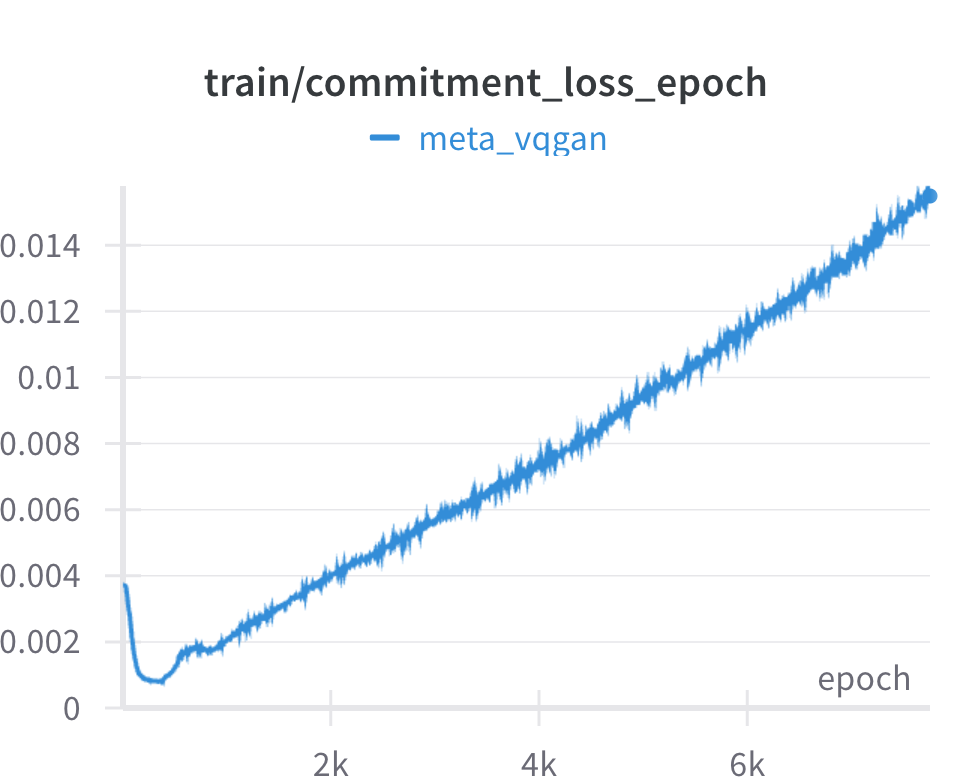
\includegraphics[width=\linewidth]{detailed_engineering/Meta VQGAN/charts/Section-2-Panel-11-4ox8mpc2c.png}
\caption{Perceptual loss during the training.}
\endminipage\hfill
\minipage{0.49\textwidth}
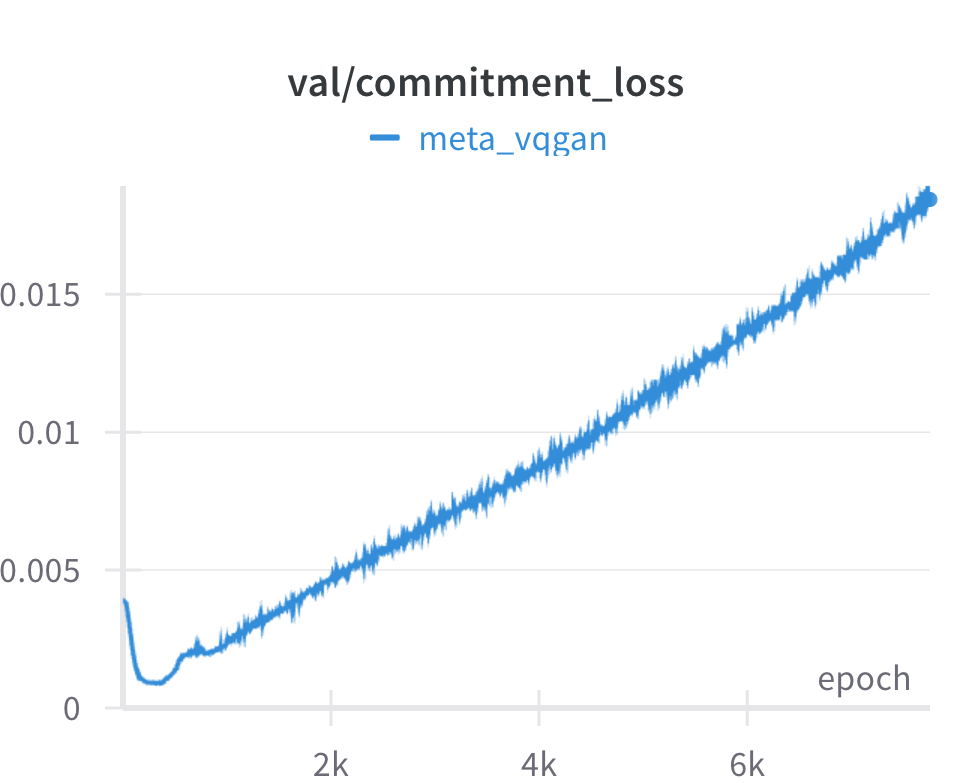
\includegraphics[width=\linewidth]{detailed_engineering/Meta VQGAN/charts/Section-4-Panel-2-2k8ixubhi.png}
\caption{Perceptual loss during the validation.}
\endminipage
\caption{Perceptual loss during the training and the validation. Lower is better.}
\end{figure}

\begin{figure}[H]
\minipage{0.49\textwidth}
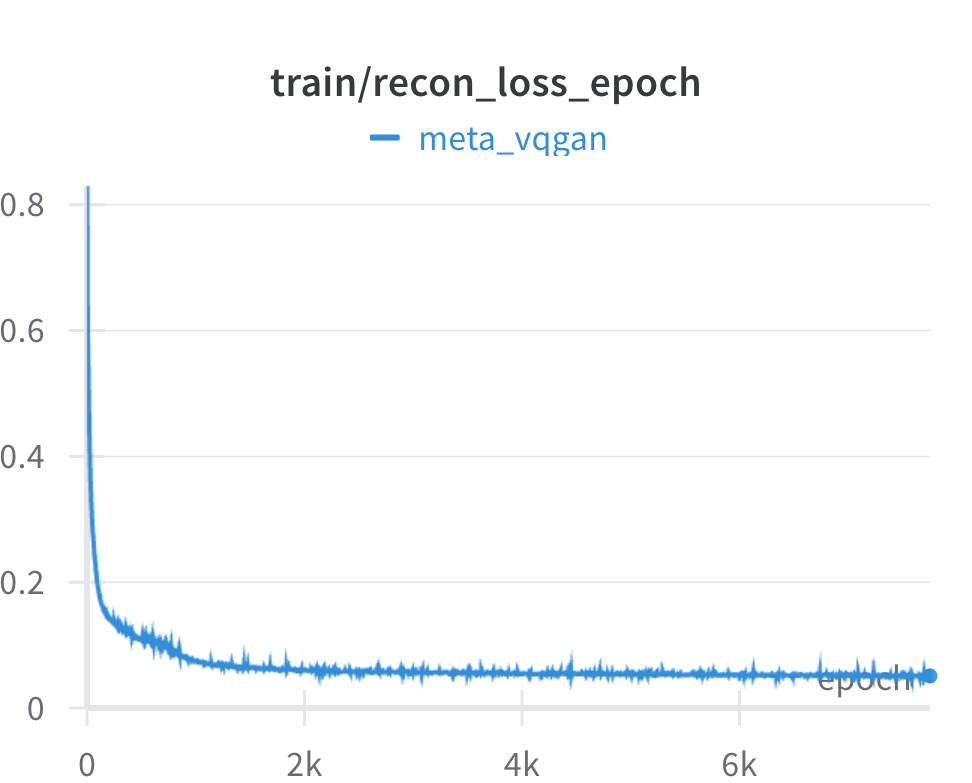
\includegraphics[width=\linewidth]{detailed_engineering/Meta VQGAN/charts/Section-2-Panel-13-1qhe42yar.png}
\caption{Commitment loss during the training.}
\endminipage\hfill
\minipage{0.49\textwidth}
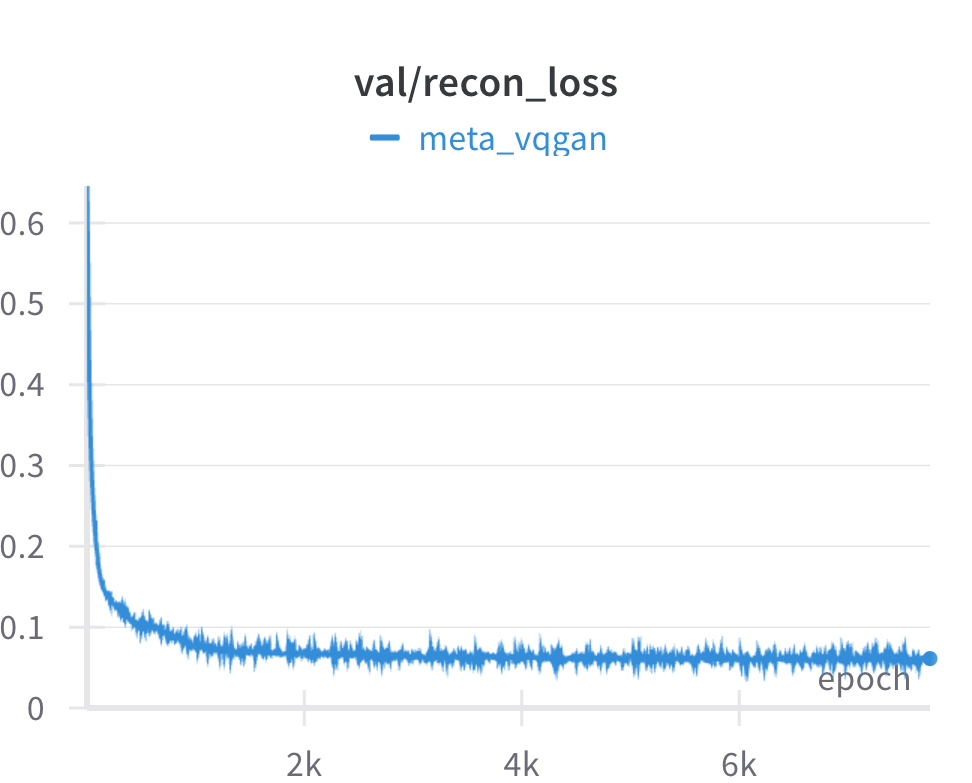
\includegraphics[width=\linewidth]{detailed_engineering/Meta VQGAN/charts/Section-4-Panel-3-hkj1c12xb.png}
\caption{Commitment loss during the validation.}
\endminipage
\caption{Commitment loss during the training and the validation. Lower is better.}
\end{figure}

\begin{figure}[H]
\minipage{0.49\textwidth}
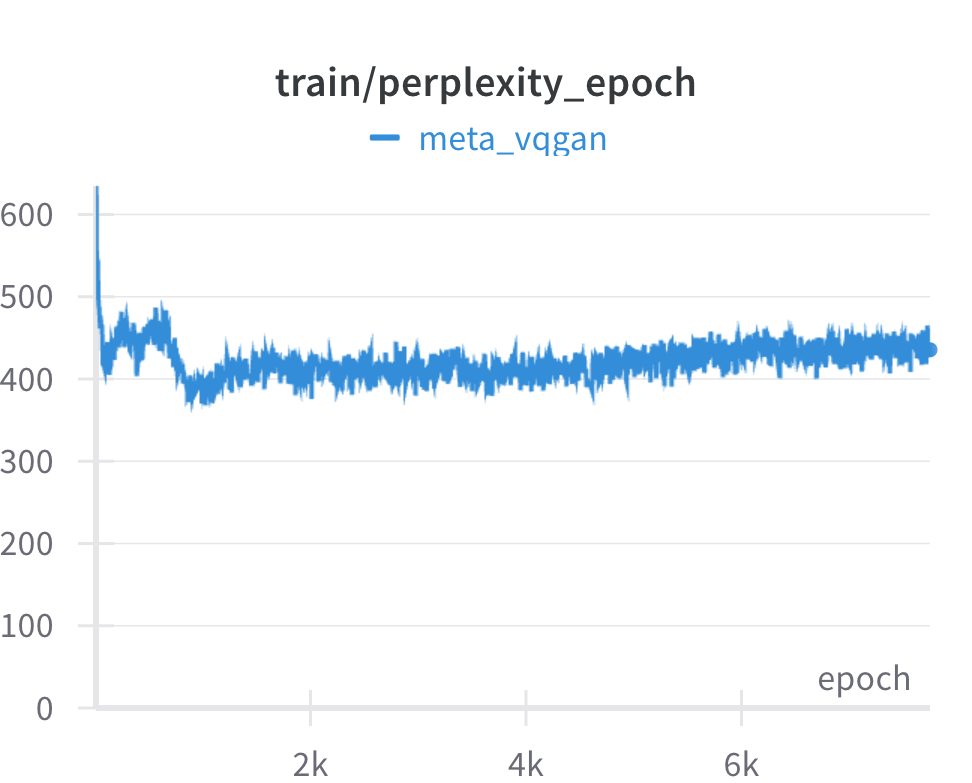
\includegraphics[width=\linewidth]{detailed_engineering/Meta VQGAN/charts/Section-2-Panel-1-5nrgzgmoj.png}
\caption{Perplexity during the training.}
\endminipage\hfill
\minipage{0.49\textwidth}
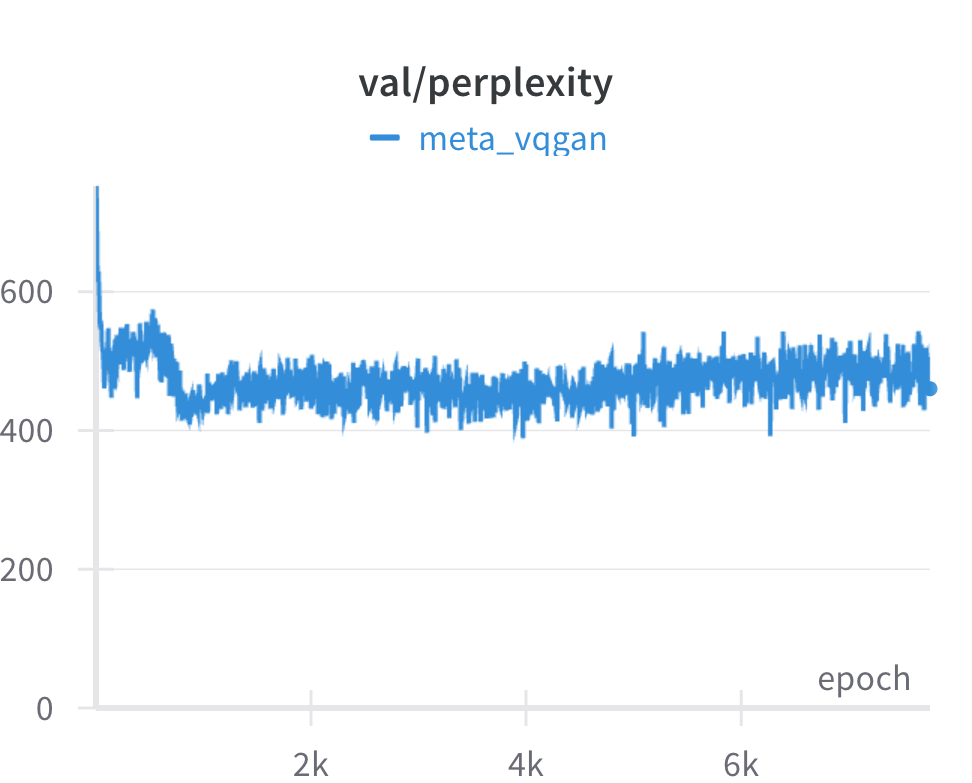
\includegraphics[width=\linewidth]{detailed_engineering/Meta VQGAN/charts/Section-4-Panel-1-njiwngfn7.png}
\caption{Perplexity during the validation.}
\endminipage
\caption{Codebook utilisation during the training and the validation. Higher is better.}
\end{figure}

\paragraph{Results}\mbox{}\\

\begin{figure}[H]
    \centering
    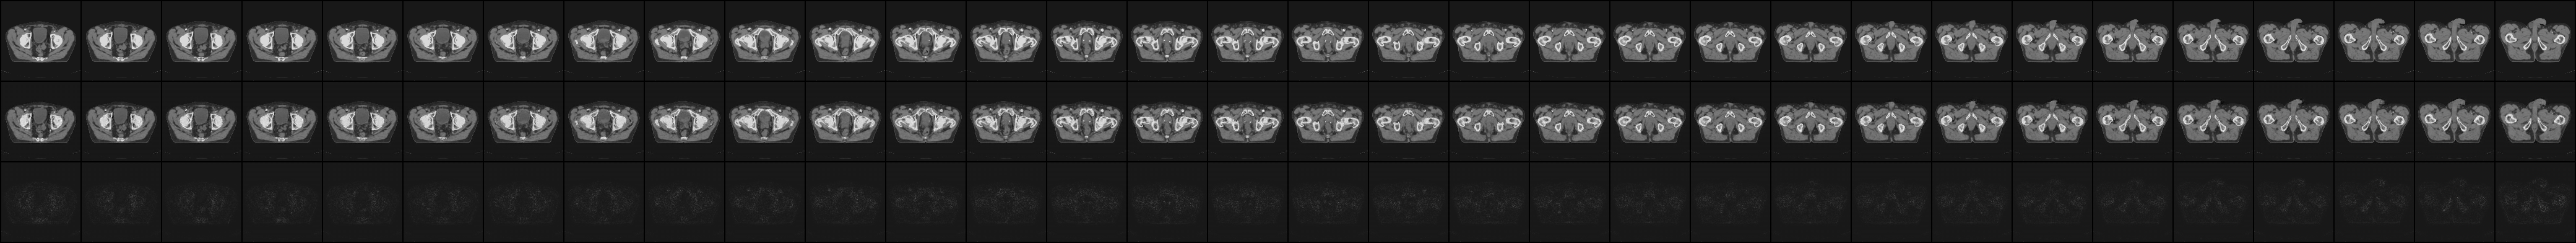
\includegraphics[width=\linewidth]{reports/meta_vqgan_reconstruction_comparison.png}
    \caption{Top - input, middle reconstruction, bottom difference.}
    \label{fig:enter-label}
\end{figure}


% \begin{figure}[H]
% \centering
% \begin{subfigure}[h]{.45\linewidth}
%     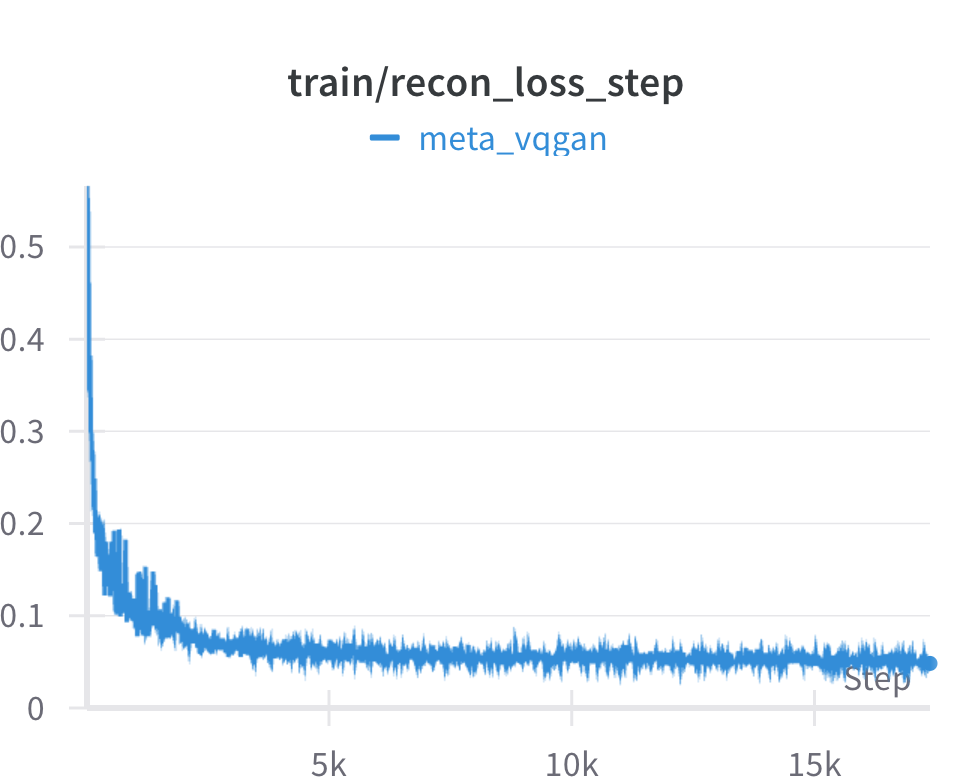
\includegraphics[width=\linewidth]{detailed_engineering/Meta VQGAN/charts/train_recon_loss_step.png}
%     \caption{Caption}
%     \label{fig:enter-label}
% \end{subfigure}
% \hfill
% \begin{subfigure}[h]{.45\linewidth}
%     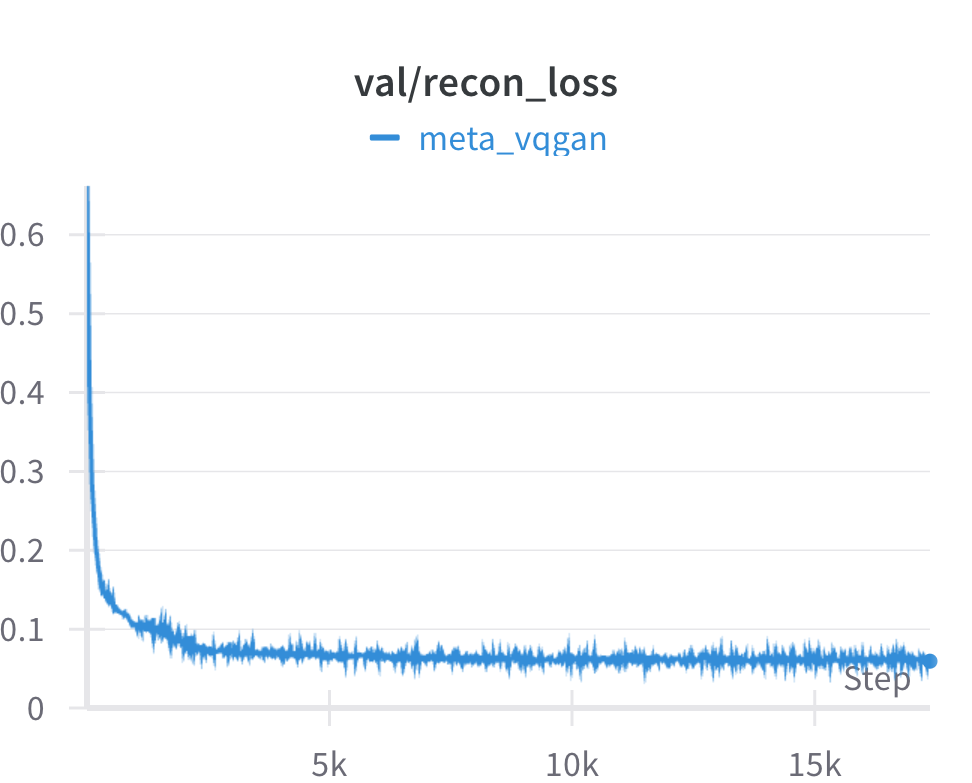
\includegraphics[width=\linewidth]{detailed_engineering/Meta VQGAN/charts/val_recon_loss.png}
%     \caption{Caption}
%     \label{fig:enter-label}
% \end{subfigure}
% \hfill
% \begin{subfigure}[h]{.45\linewidth}
%     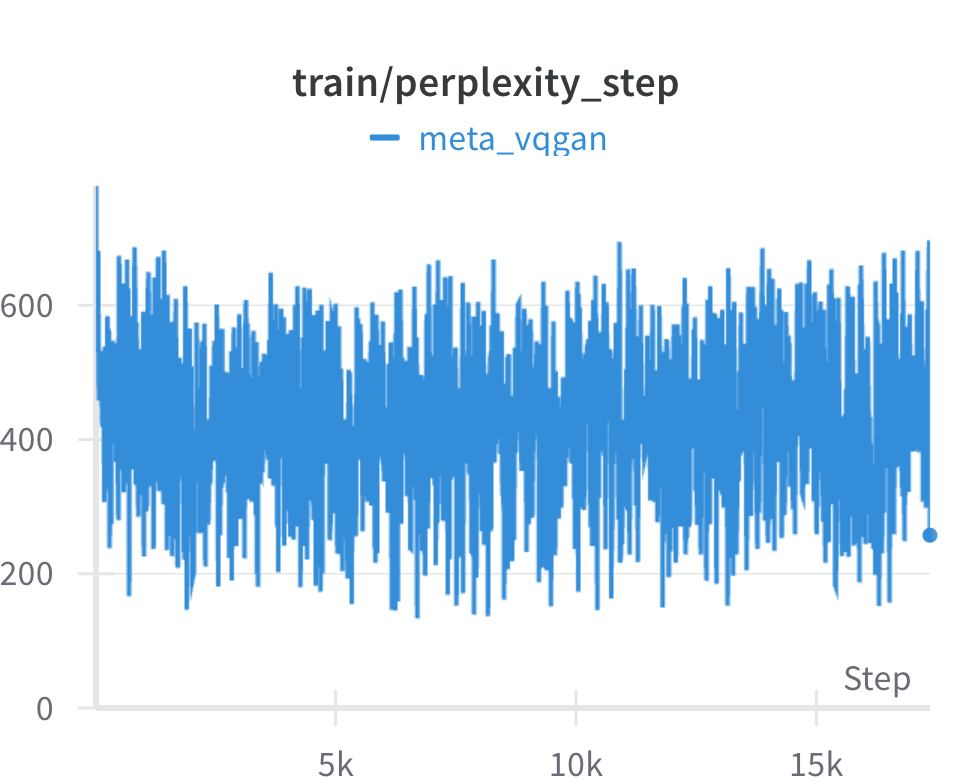
\includegraphics[width=\linewidth]{detailed_engineering/Meta VQGAN/charts/train_perplexity_step.png}
%     \caption{Caption}
%     \label{fig:enter-label}
% \end{subfigure}
% \hfill
% \begin{subfigure}[h]{.45\linewidth}
%     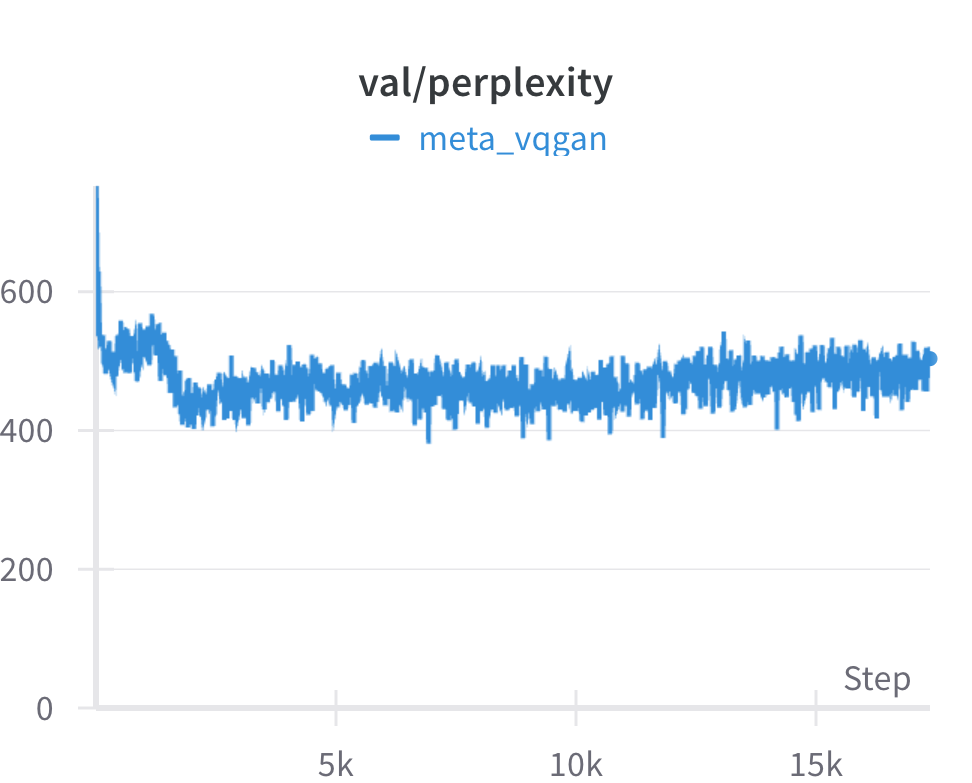
\includegraphics[width=\linewidth]{detailed_engineering/Meta VQGAN/charts/val_perplexity.png}
%     \caption{Caption}
%     \label{fig:enter-label}
% \end{subfigure}
% \hfill
% \begin{subfigure}[h]{.45\linewidth}
%     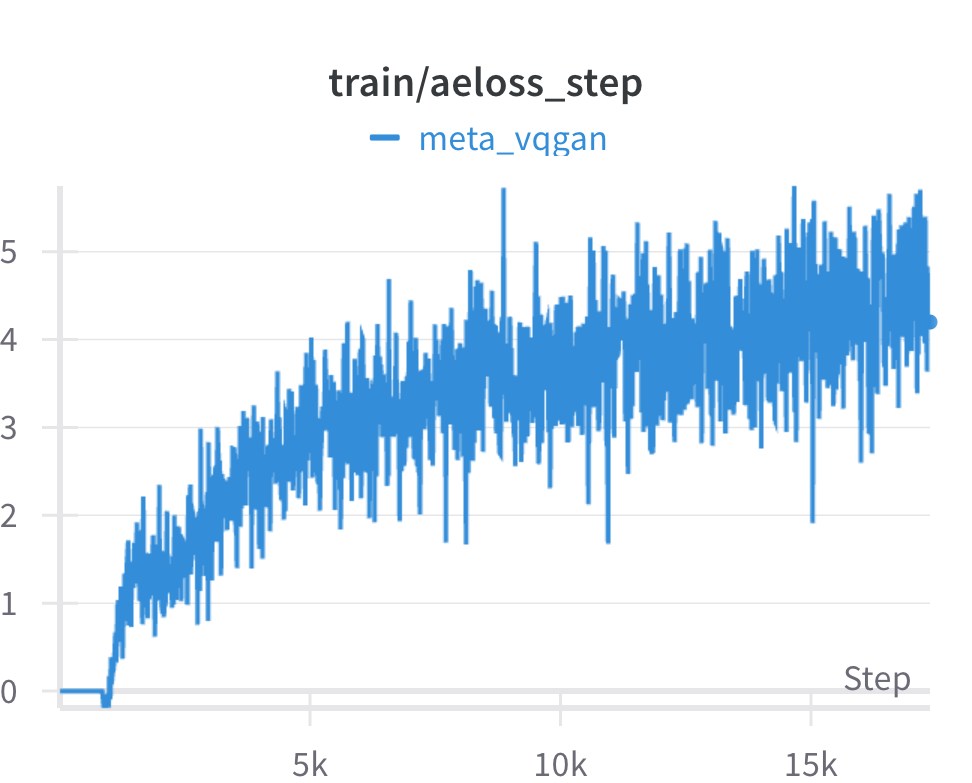
\includegraphics[width=\linewidth]{detailed_engineering/Meta VQGAN/charts/train_aeloss_step.png}
%     \caption{Caption}
%     \label{fig:enter-label}
% \end{subfigure}
% \hfill
% \begin{subfigure}[h]{.45\linewidth}
%     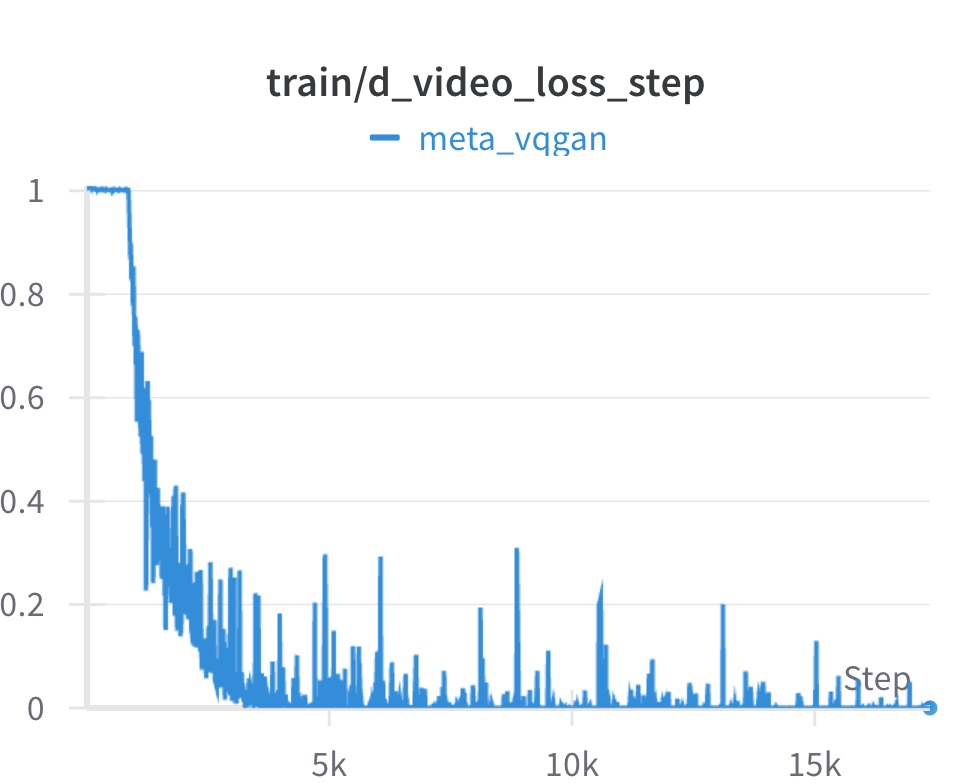
\includegraphics[width=\linewidth]{detailed_engineering/Meta VQGAN/charts/train_d_video_loss_step.png}
%     \caption{Caption}
%     \label{fig:enter-label}
% \end{subfigure}
% \hfill
% \begin{subfigure}[h]{.45\linewidth}
%     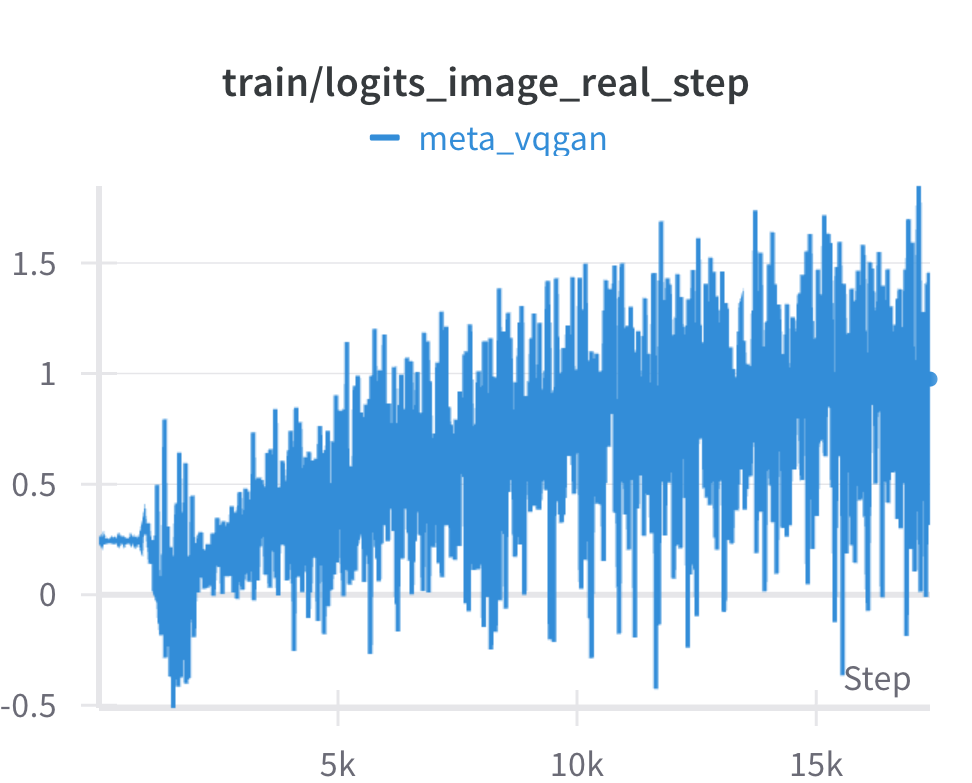
\includegraphics[width=\linewidth]{detailed_engineering/Meta VQGAN/charts/train_logits_image_real_step.png}
%     \caption{Caption}
%     \label{fig:enter-label}
% \end{subfigure}
% \hfill
% \begin{subfigure}[h]{.45\linewidth}
%     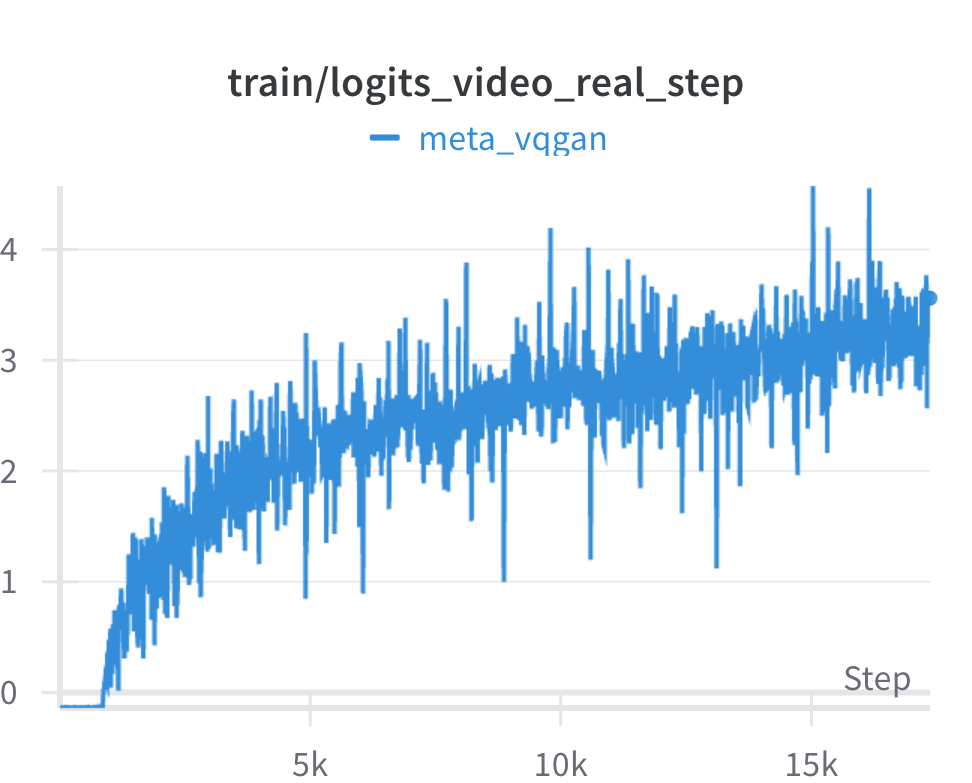
\includegraphics[width=\linewidth]{detailed_engineering/Meta VQGAN/charts/train_logits_video_real_step.png}
%     \caption{Caption}
%     \label{fig:enter-label}
% \end{subfigure}
% \hfill
% \begin{subfigure}[h]{.45\linewidth}
%     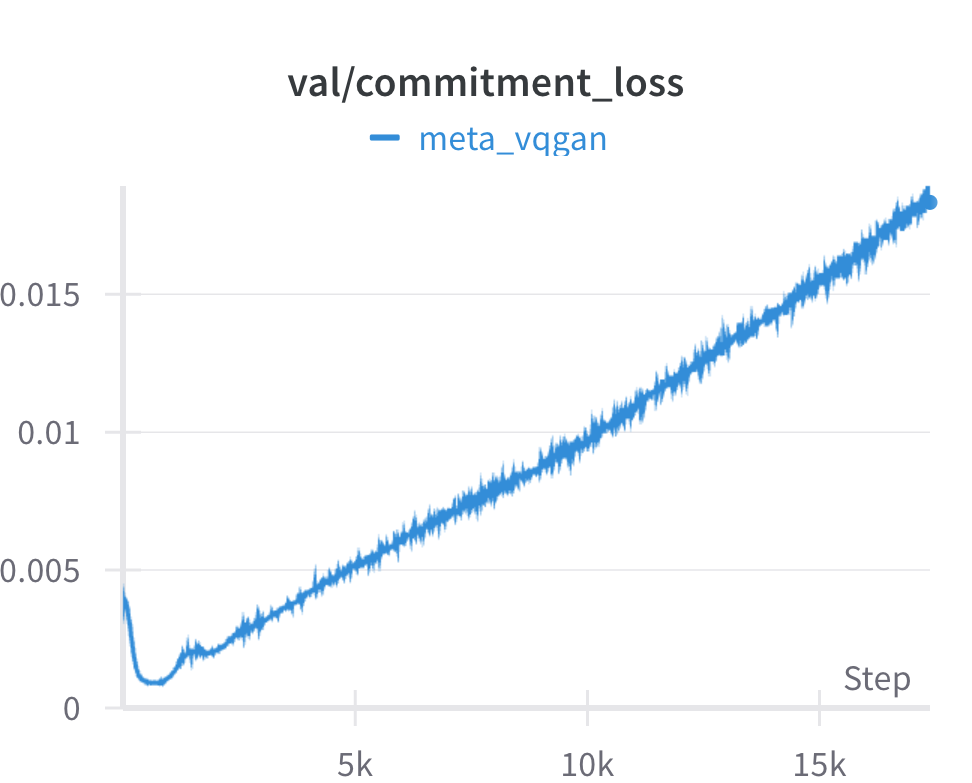
\includegraphics[width=\linewidth]{detailed_engineering/Meta VQGAN/charts/val_commitment_loss.png}
%     \caption{Caption}
%     \label{fig:enter-label}
% \end{subfigure}
% \hfill
% \begin{subfigure}[h]{.45\linewidth}
%     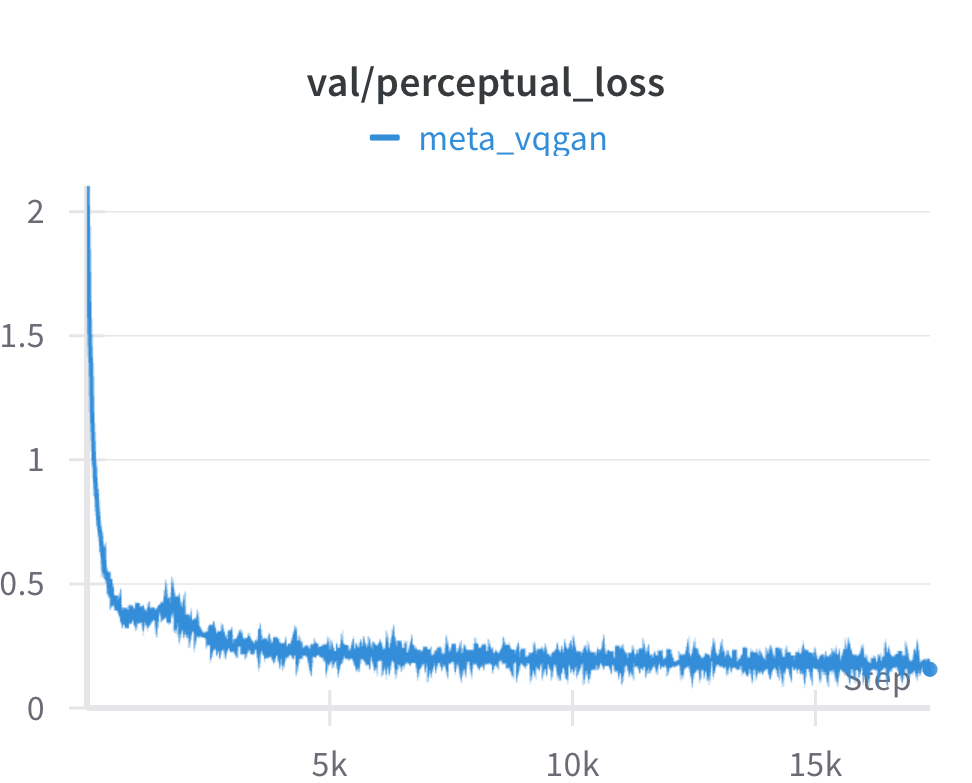
\includegraphics[width=\linewidth]{detailed_engineering/Meta VQGAN/charts/val_perceptual_loss.png}
%     \caption{Caption}
%     \label{fig:enter-label}
% \end{subfigure}
% \end{figure}


\paragraph{Results}

\newpage
\paragraph{Medical Diffusion LDM}\mbox{}\\


\begin{figure}[H]
\minipage{0.49\textwidth}
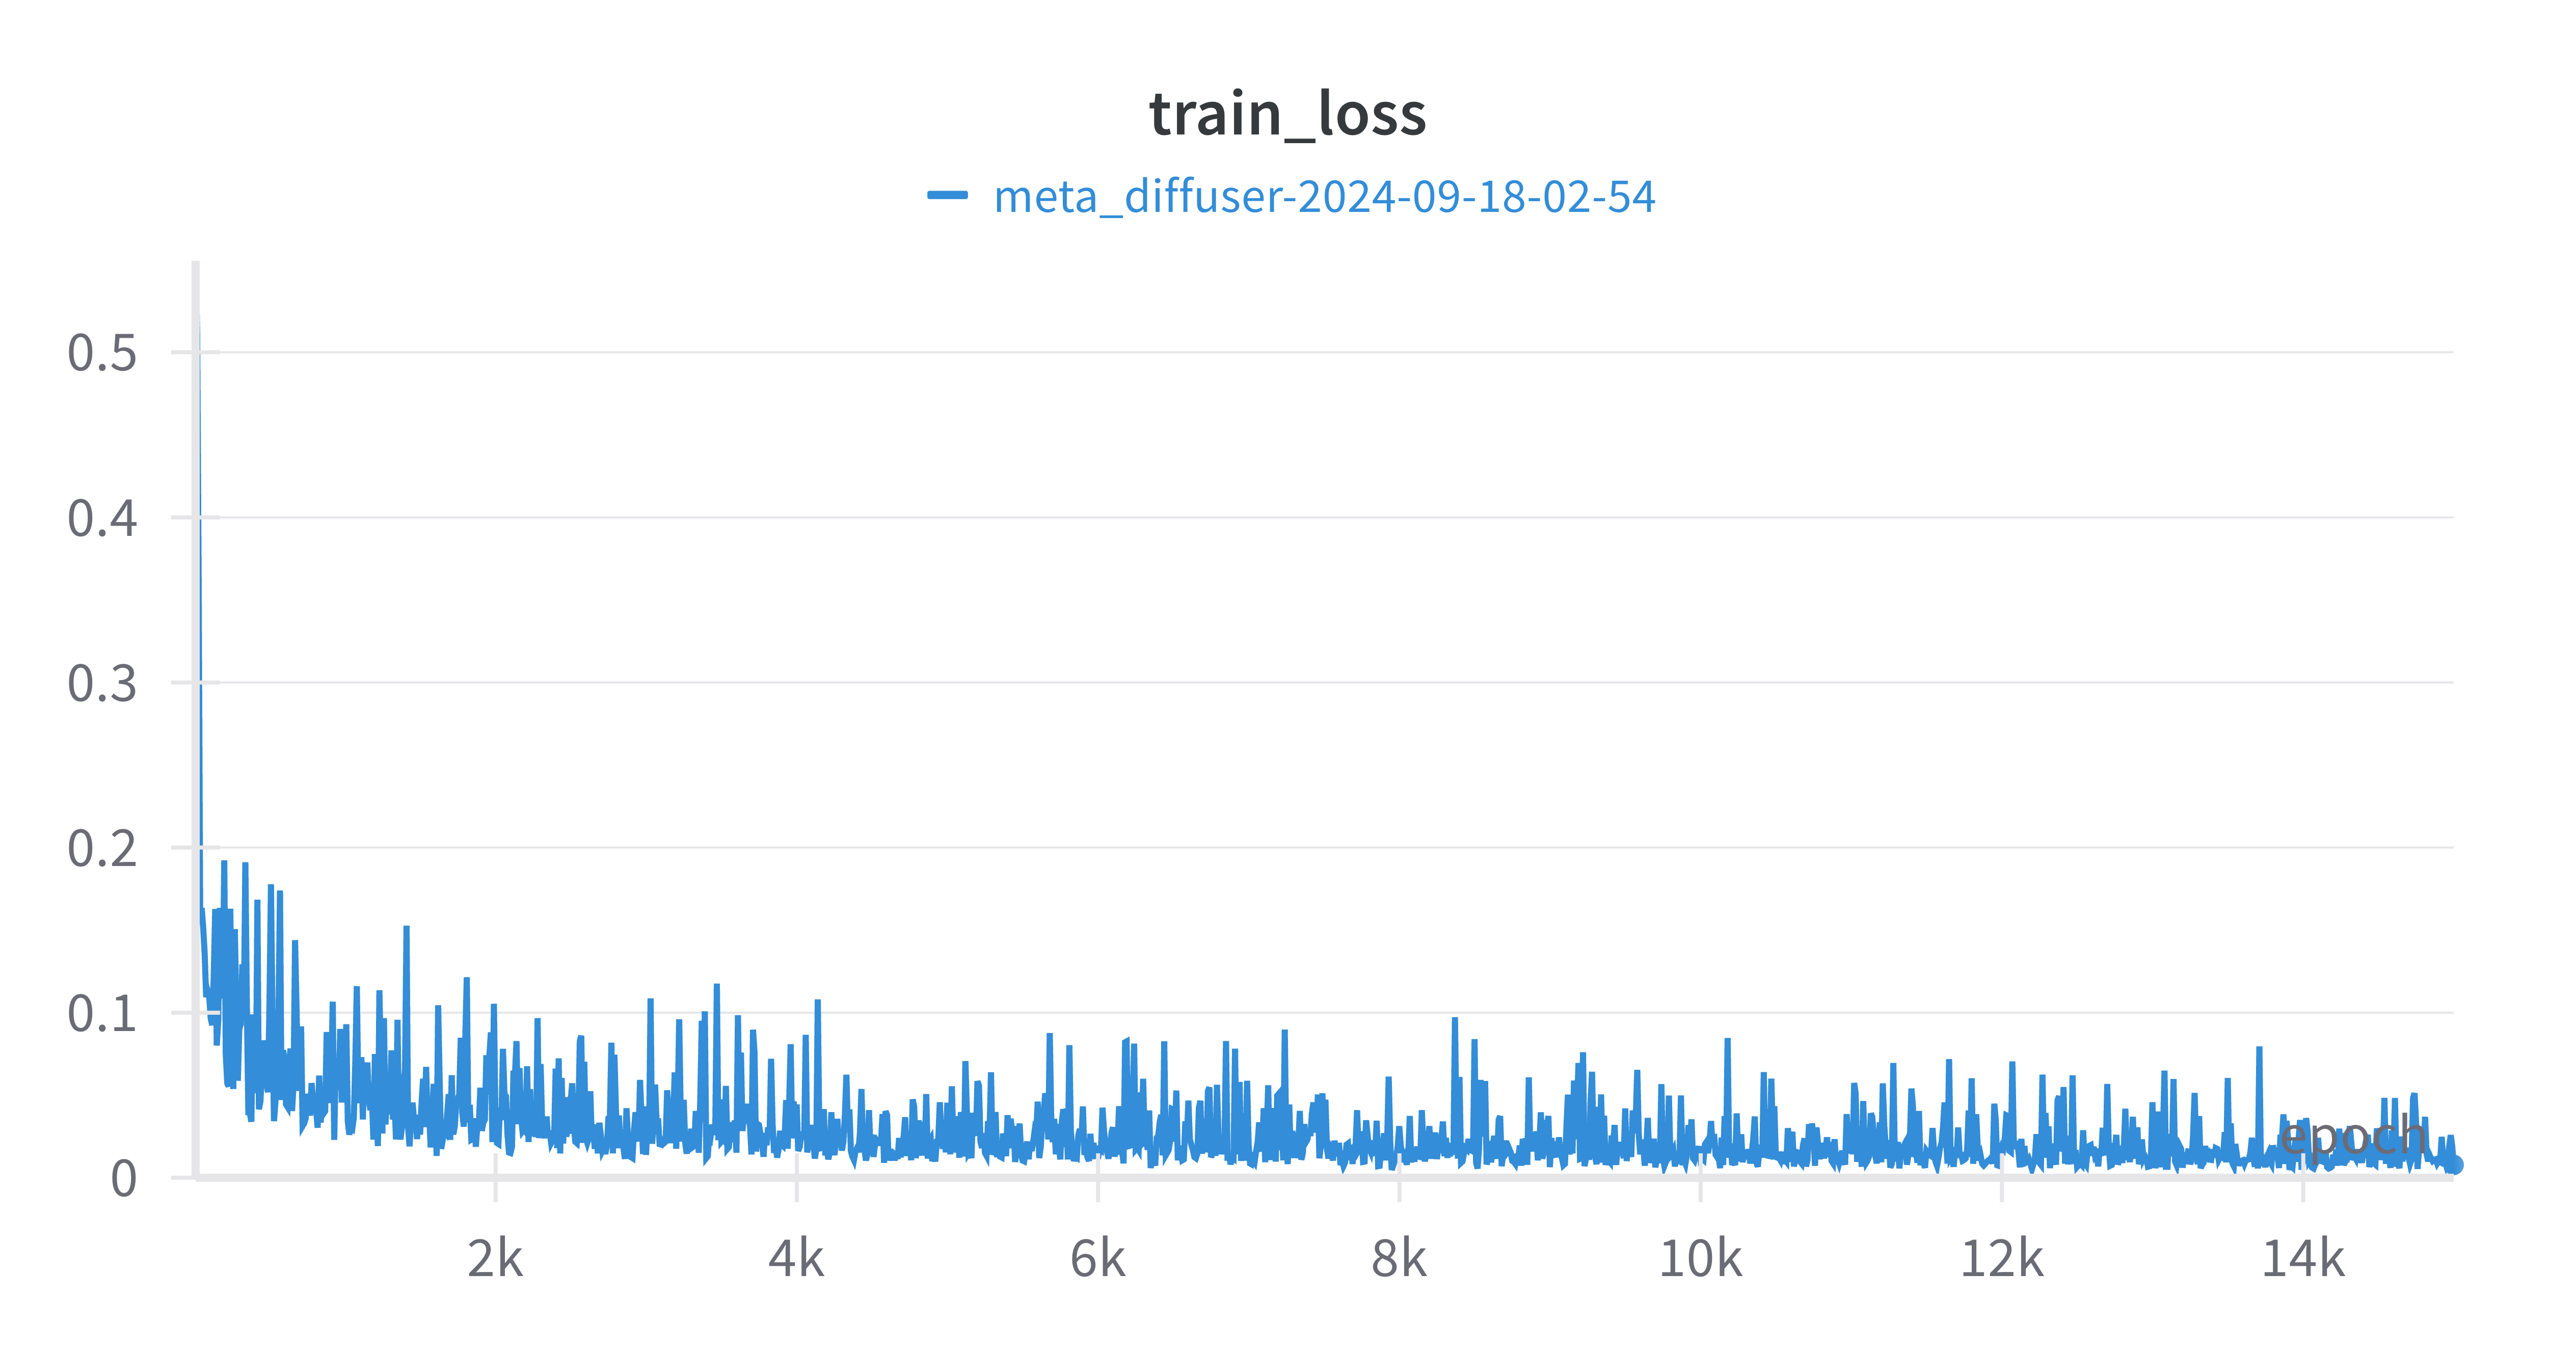
\includegraphics[width=\linewidth]{detailed_engineering/Meta Diffusion/charts/train_loss.png}
\caption{Loss during the training. Lower is better.}
\endminipage\hfill
\minipage{0.49\textwidth}
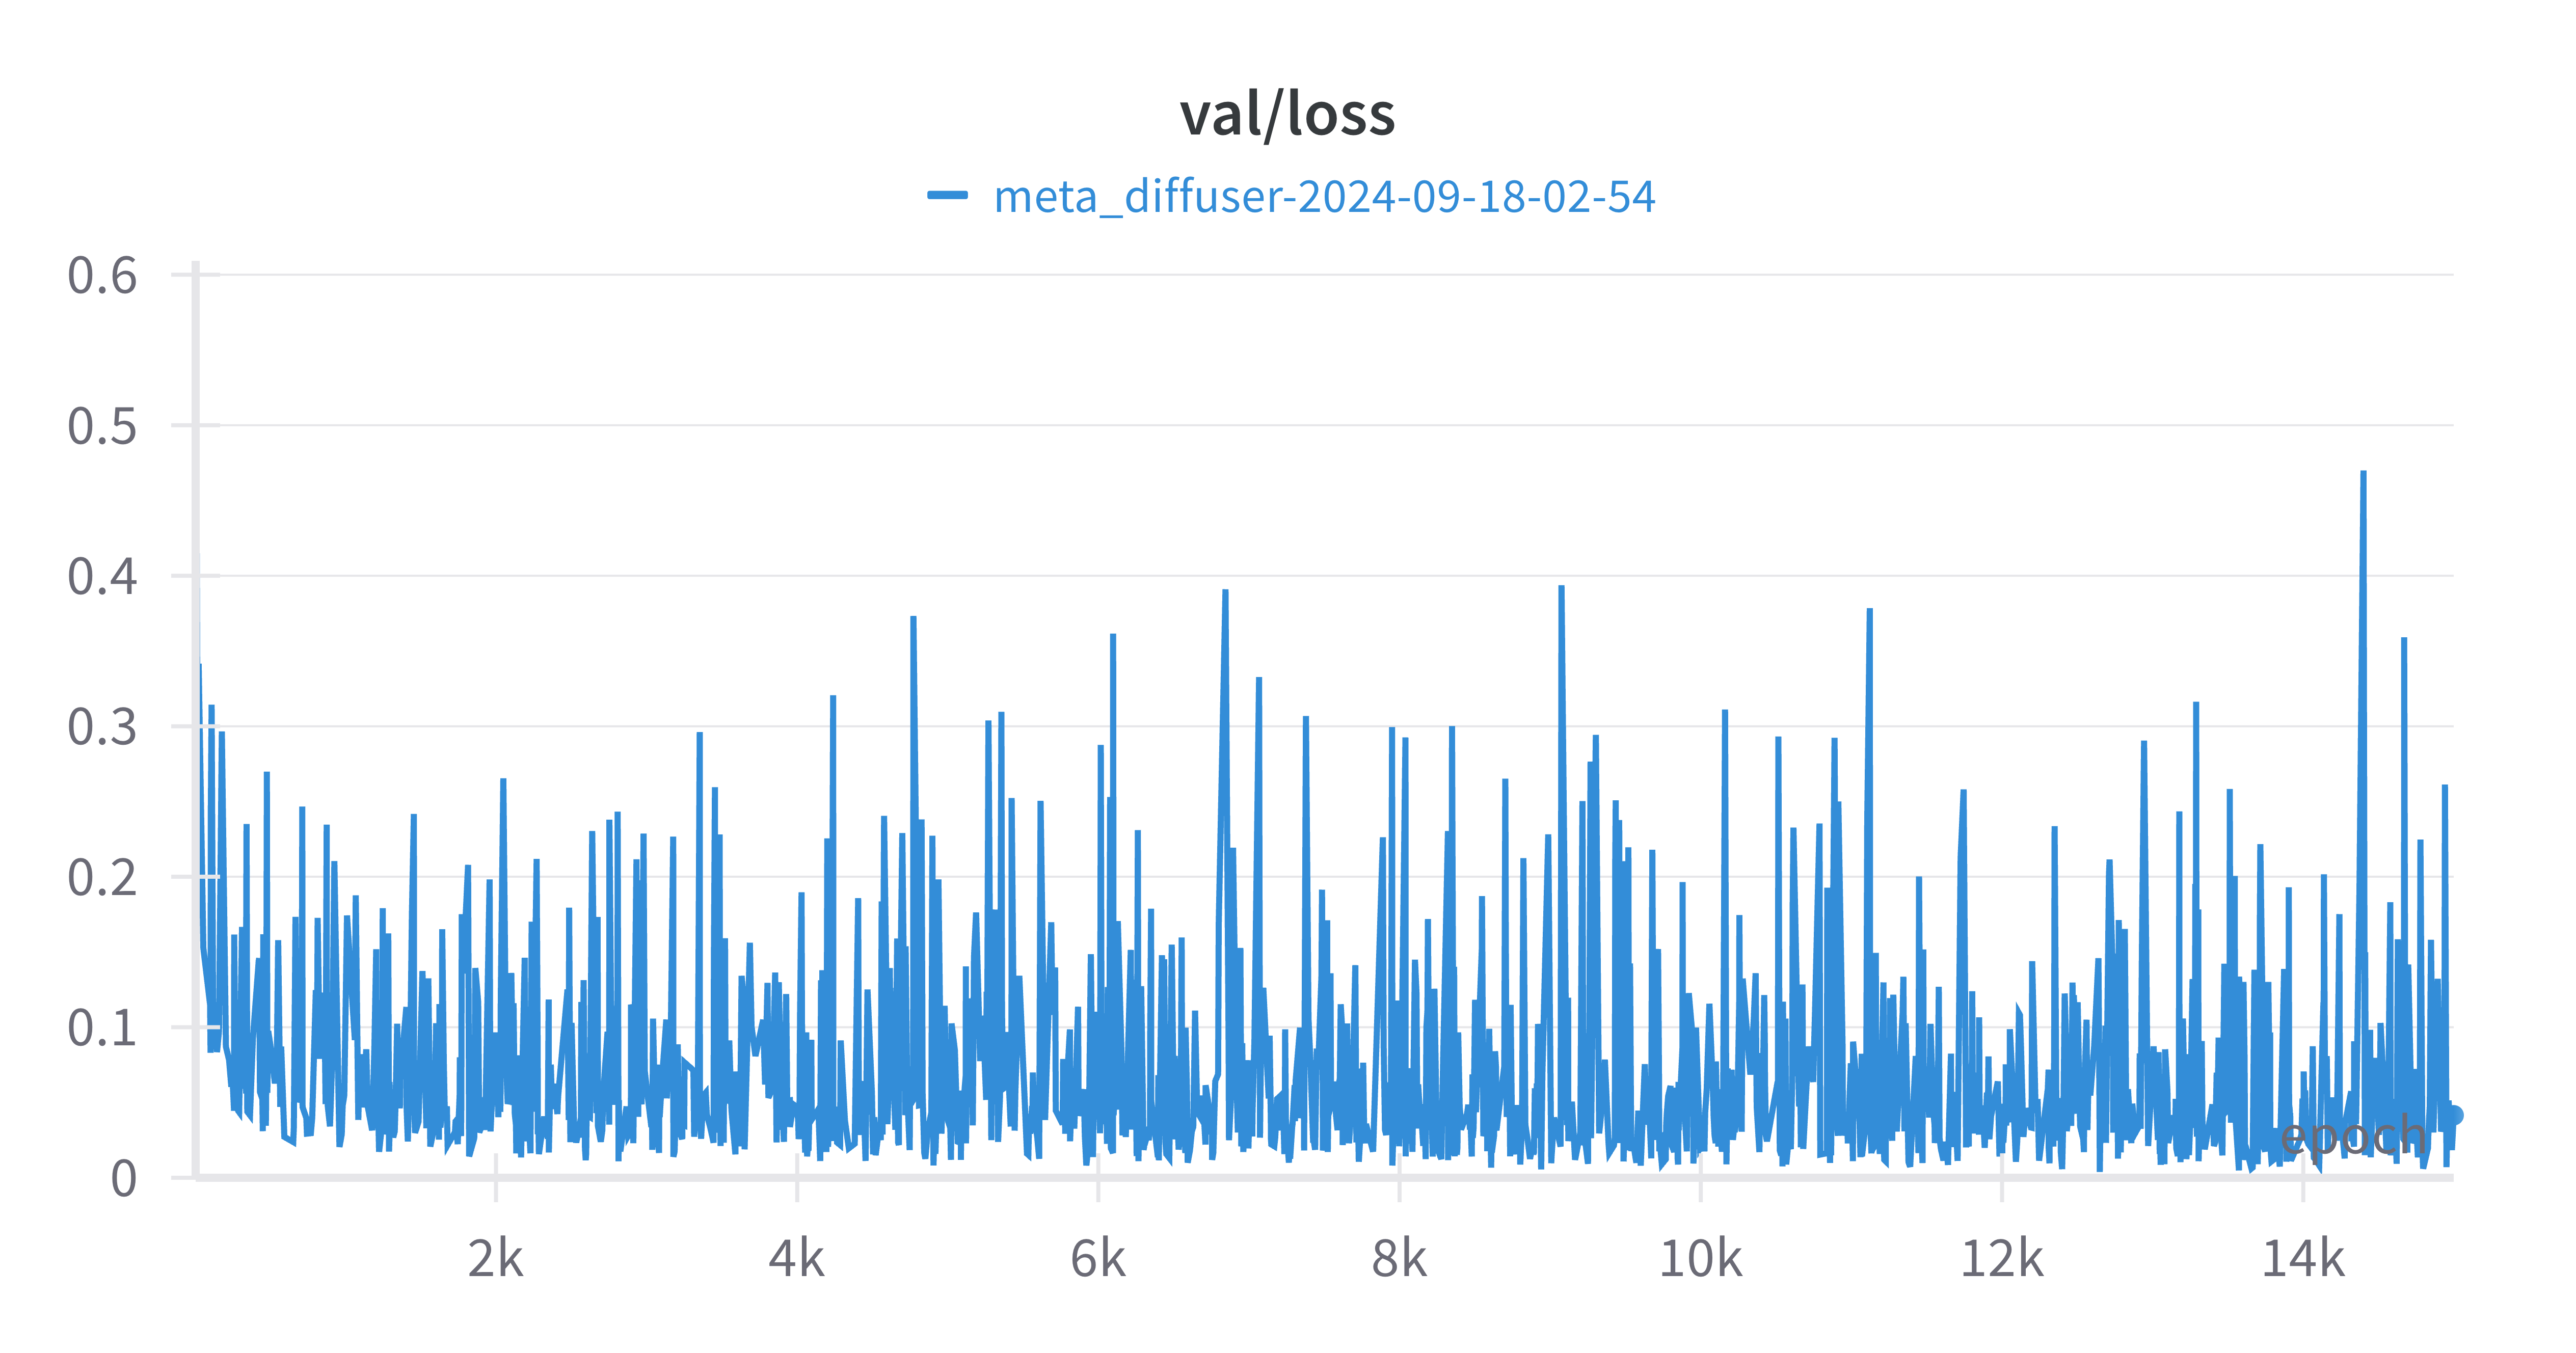
\includegraphics[width=\linewidth]{detailed_engineering/Meta Diffusion/charts/val_loss.png}
\caption{Loss during the validation. Lower is better.}
\endminipage
\end{figure}

Additional metrics evaluating the quality of the generated scan.
\begin{figure}[H]
\minipage{0.49\textwidth}
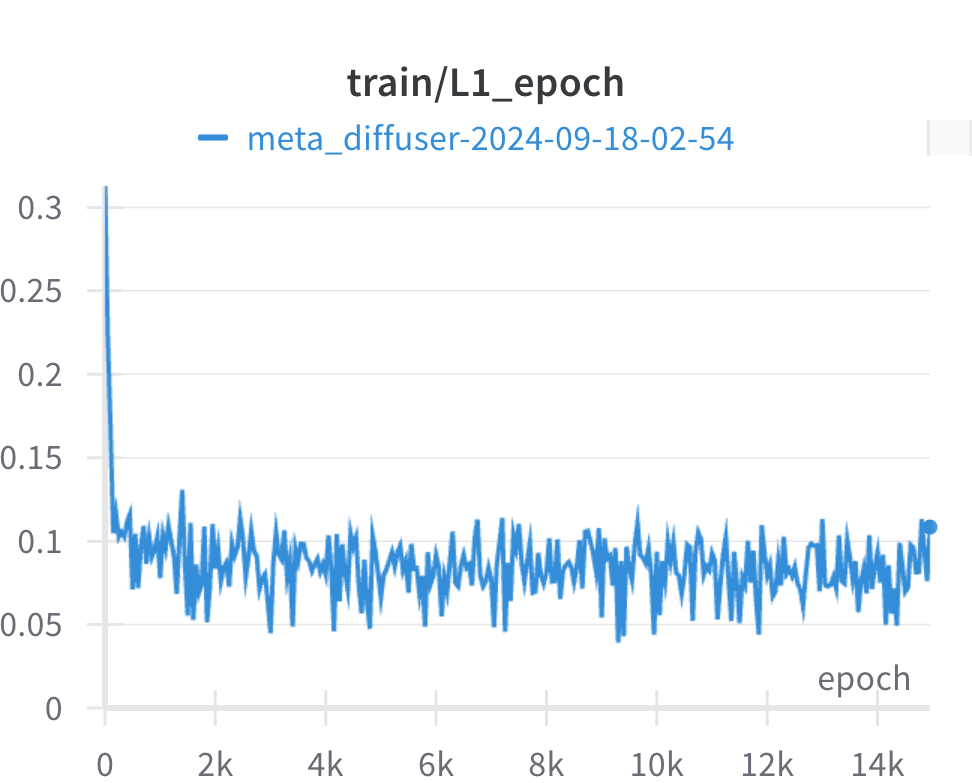
\includegraphics[width=\linewidth]{detailed_engineering/Meta Diffusion/charts/train_l1_epoch.png}

\endminipage\hfill
\minipage{0.49\textwidth}
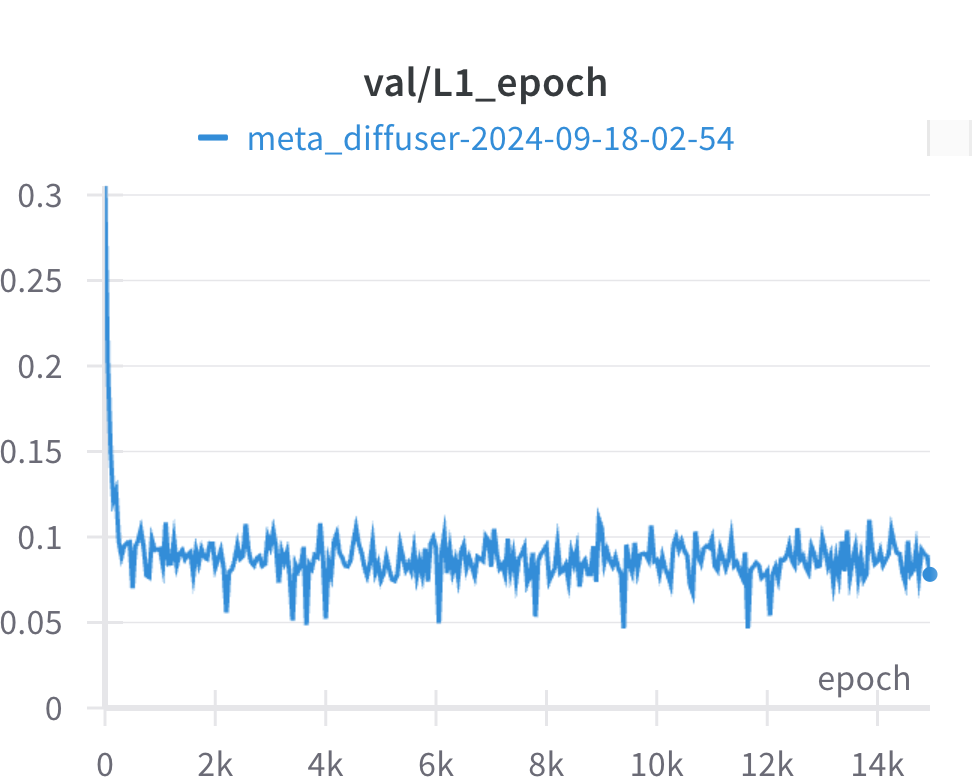
\includegraphics[width=\linewidth]{detailed_engineering/Meta Diffusion/charts/val_l1_epoch.png}

\endminipage
\caption{L1 between two generated CT scans and two random samples from training/validation datasets. Lower is better.}
\end{figure}

\begin{figure}[H]
\minipage{0.49\textwidth}
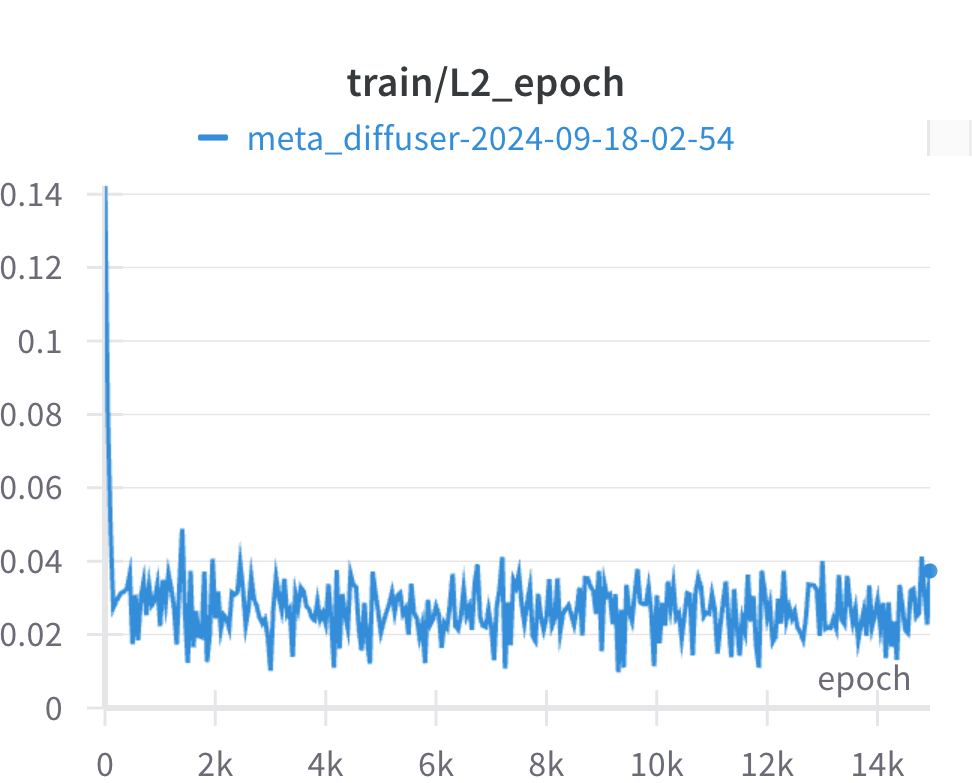
\includegraphics[width=\linewidth]{detailed_engineering/Meta Diffusion/charts/train_l2_epoch.png}

\endminipage\hfill
\minipage{0.49\textwidth}
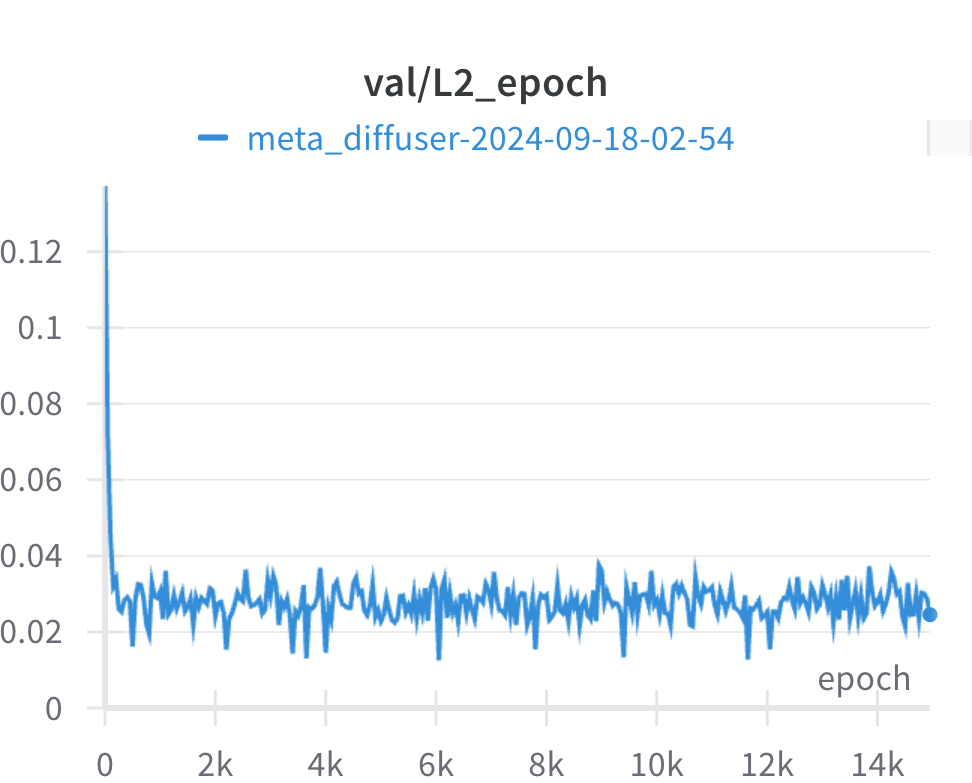
\includegraphics[width=\linewidth]{detailed_engineering/Meta Diffusion/charts/val_l2_epoch.png}

\endminipage
\caption{L2 between two generated CT scasn and two random samples from training/validation datasets. Lower is better.}
\end{figure}

\begin{figure}[H]
\minipage{0.49\textwidth}
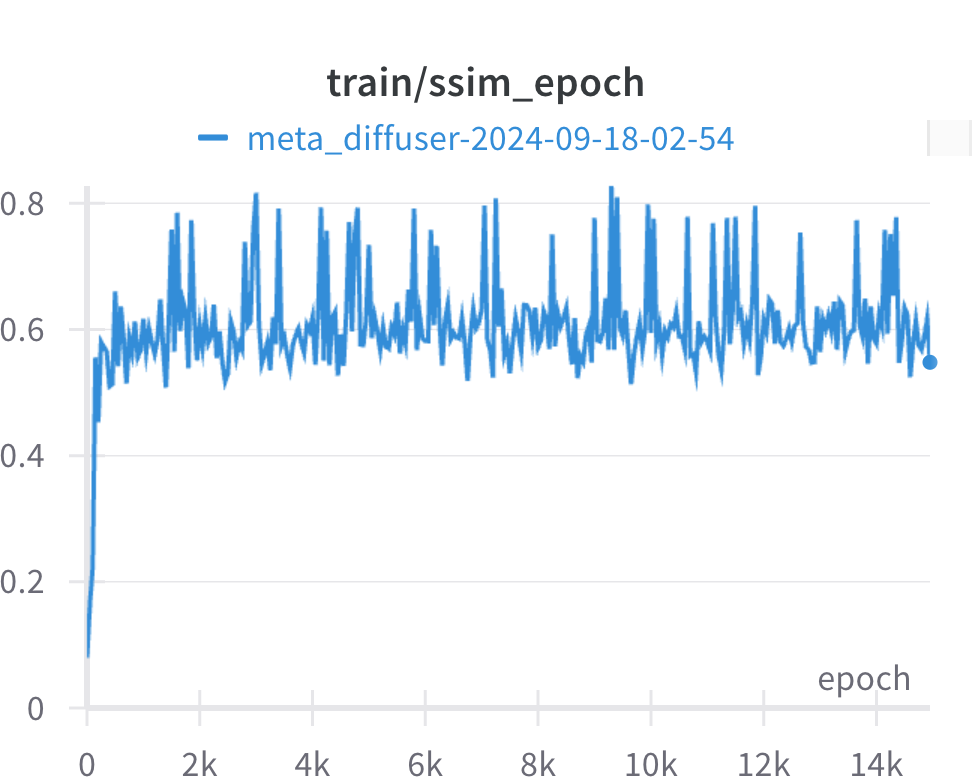
\includegraphics[width=\linewidth]{detailed_engineering/Meta Diffusion/charts/train_ssim_epoch.png}

\endminipage\hfill
\minipage{0.49\textwidth}
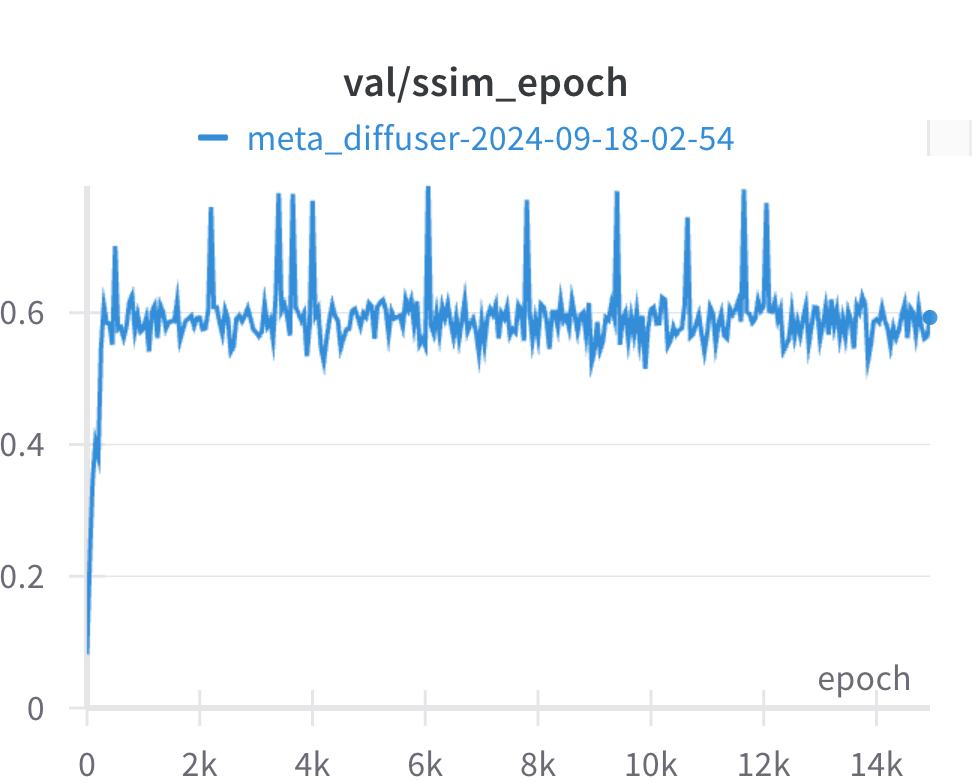
\includegraphics[width=\linewidth]{detailed_engineering/Meta Diffusion/charts/val_ssim_epoch.png}

\endminipage
\caption{MSSIM between two generated Ct scans and two random samples from training/validation datasets. Higher is better.}
\end{figure}

\paragraph{Results}\mbox{}\\

% \begin{figure}[H]
%     \centering
%     \includegraphics[width=\linewidth]{}
%     \caption{Caption}
%     \label{fig:enter-label}
% \end{figure}
\begin{figure}[H]
    \centering
    % \includegraphics{}
     \animategraphics[width=\textwidth, loop, autoplay]{5}%frame rate
    {detailed_engineering/Meta Diffusion/generation/layer-}%path to figures
    {0}%start index
    {31}%end index
    \caption{Random layer of synthetic CT scan generated from Gaussian noise.}
    \label{fig:my_label}
\end{figure}

\begin{figure}[H]
    \centering
    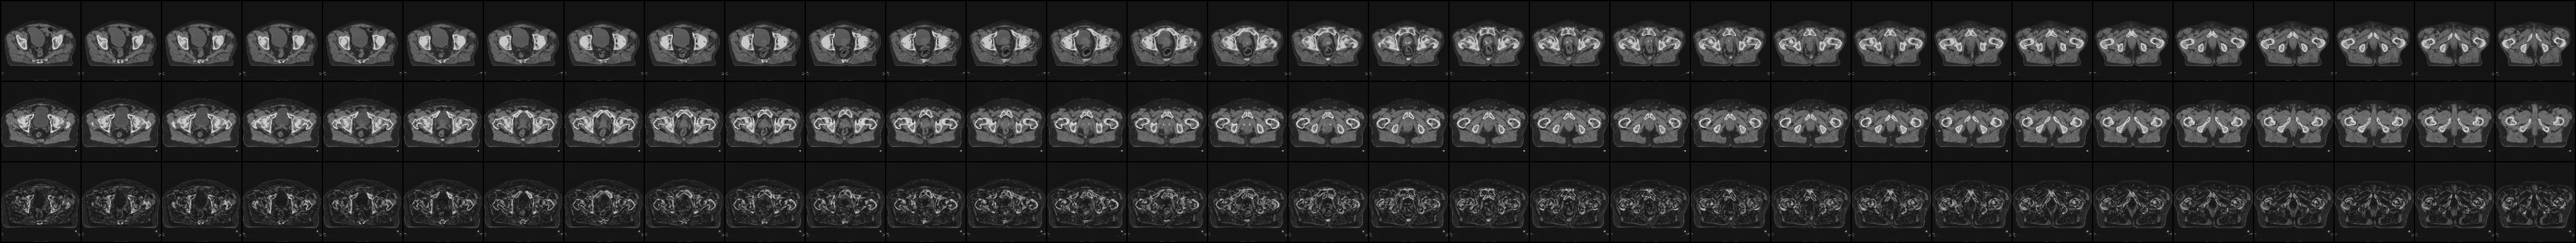
\includegraphics[width=\linewidth]{detailed_engineering/Meta Diffusion/charts/meta_diffusion_comparison.png}
    \caption{Top - first sample from trianing dataset, middle - synthetic CT scan, bottom - L1 difference between them.}
    \label{fig:enter-label}
\end{figure}

\paragraph{Model configuration}

% \paragraph{Training}
% \begin{figure}[H]
% \centering
% \begin{subfigure}[h]{.45\linewidth}
%     \includegraphics[width=\linewidth]{detailed_engineering/}
%     \caption{Caption}
%     \label{fig:enter-label}
% \end{subfigure}
% \hfill
% \begin{subfigure}[h]{.45\linewidth}
%     \includegraphics[width=\linewidth]{detailed_engineering/Monai Autoencoder/charts/Section-4-Panel-2-bm1y05a9m.png}
%     \caption{Caption}
%     \label{fig:enter-label}
% \end{subfigure}
% \hfill
% \begin{subfigure}[h]{.45\linewidth}
%     \includegraphics[width=\linewidth]{detailed_engineering/Monai Autoencoder/charts/Section-4-Panel-3-dkwhik6ki.png}
%     \caption{Caption}
%     \label{fig:enter-label}
% \end{subfigure}
% \hfill
% \begin{subfigure}[h]{.45\linewidth}
%     \includegraphics[width=\linewidth]{detailed_engineering/Monai Autoencoder/charts/Section-4-Panel-4-d216pe2qa.png}
%     \caption{Caption}
%     \label{fig:enter-label}
% \end{subfigure}
% \hfill
% \begin{subfigure}[h]{.45\linewidth}
%     \includegraphics[width=\linewidth]{detailed_engineering/Monai Autoencoder/charts/Section-4-Panel-5-z2xepgyu7.png}
%     \caption{Caption}
%     \label{fig:enter-label}
% \end{subfigure}
% \end{figure}


\paragraph{Results}
